\documentclass[a4paper,11pt]{article}
\usepackage[utf8]{inputenc} % Sonderzeichen schreiben können
\usepackage[ngerman]{babel} % Deutsche Abbildungszeichen
\usepackage{graphicx}   % Graphiken einfügen
\usepackage{fancyhdr}   % Für Kopf- und Fusszeile
\usepackage{geometry}   % Seitenränder definieren
\usepackage{tikz}       % Zum Regler zeichnen
\usepackage{multirow}   % Multirow in Tabellen
\usepackage{float}      % Um Bilder genau an diesem Punkt einzufuegen [H]
\usepackage{fancyvrb}   % Box um Verbatim Code
\usepackage{microtype}  % Automatische Anpassung der Zeilenmaße, dass unschöne Umbrüche vermieden werden
\usepackage{mathtools}  % Für Text auf/unter Pfeilen
\usepackage{pgfplots}   % Plot zusammen mit tikzpicture
\usepackage{makecell}   % Umbruch in tabellen
\usepackage{enumitem}   % Einruecken bei itemize verhindern
\usepackage{titlesec}   % Elemente unter subsubsection erzeugen
\usepackage{trfsigns}   % Transformationssymbole
\usepackage{amsmath}    % Umbruch in Formeln
\usepackage{listings}   % Code darstellen
\usepackage{xcolor}     % Code farbig machen
\usepackage{longtable}  % Tabellen mit Seitenumbruch
\usepackage{textcomp}
\usepackage{url}
\usepackage[font=footnotesize, labelfont=bf]{caption}
\usetikzlibrary{shapes,arrows}
\pgfplotsset{compat = newest}

\usepackage[colorlinks,
pdfpagelabels,
pdfstartview = FitH,
bookmarksopen = true,
bookmarksnumbered = true,
linkcolor = black,
plainpages = false,
hypertexnames = false,
citecolor = black] {hyperref}

% Seitenränder definieren
\geometry{
    left=25mm,
    right=25mm,
    top=25mm,
    %bottom=25mm
    }
    
\definecolor{codegreen}{rgb}{0,0.6,0}
\definecolor{codegray}{rgb}{0.5,0.5,0.5}
\definecolor{codepurple}{rgb}{0.58,0,0.82}
\definecolor{backcolour}{rgb}{0.95,0.95,0.92}

\lstdefinestyle{mystyle}{
    backgroundcolor=\color{backcolour},   
    commentstyle=\color{codegreen},
    keywordstyle=\color{magenta},
    numberstyle=\tiny\color{codegray},
    stringstyle=\color{codepurple},
    basicstyle=\ttfamily\footnotesize,
    breakatwhitespace=false,         
    breaklines=true,                 
    captionpos=b,                    
    keepspaces=true,                 
    numbers=left,                    
    numbersep=5pt,                  
    showspaces=false,                
    showstringspaces=false,
    showtabs=false,                  
    tabsize=2
}

\lstset{style=mystyle}

\titleclass{\subsubsubsection}{straight}[\subsection]

\newcounter{subsubsubsection}[subsubsection]
\renewcommand\thesubsubsubsection{\thesubsubsection.\arabic{subsubsubsection}}
\renewcommand\theparagraph{\thesubsubsubsection.\arabic{paragraph}} % optional; useful if paragraphs are to be numbered

\titleformat{\subsubsubsection}
  {\normalfont\normalsize\bfseries}{\thesubsubsubsection}{1em}{}
\titlespacing*{\subsubsubsection}
{0pt}{3.25ex plus 1ex minus .2ex}{1.5ex plus .2ex}

\makeatletter
\renewcommand\paragraph{\@startsection{paragraph}{5}{\z@}%
  {3.25ex \@plus1ex \@minus.2ex}%
  {-1em}%
  {\normalfont\normalsize\bfseries}}
\renewcommand\subparagraph{\@startsection{subparagraph}{6}{\parindent}%
  {3.25ex \@plus1ex \@minus .2ex}%
  {-1em}%
  {\normalfont\normalsize\bfseries}}
\def\toclevel@subsubsubsection{4}
\def\toclevel@paragraph{5}
\def\toclevel@paragraph{6}
\def\l@subsubsubsection{\@dottedtocline{4}{7em}{4em}}
\def\l@paragraph{\@dottedtocline{5}{10em}{5em}}
\def\l@subparagraph{\@dottedtocline{6}{14em}{6em}}
\makeatother

\setcounter{secnumdepth}{4}
\setcounter{tocdepth}{4}

\newenvironment{nospaceflalign*}
 {\setlength{\abovedisplayskip}{0pt}\setlength{\belowdisplayskip}{0pt}%
  \csname flalign*\endcsname}
 {\csname endflalign*\endcsname\ignorespacesafterend}

\pagestyle{fancy}
\fancyhf{}
\setlength{\headheight}{28.1pt} % Höhe der Kopfzeile
\rhead{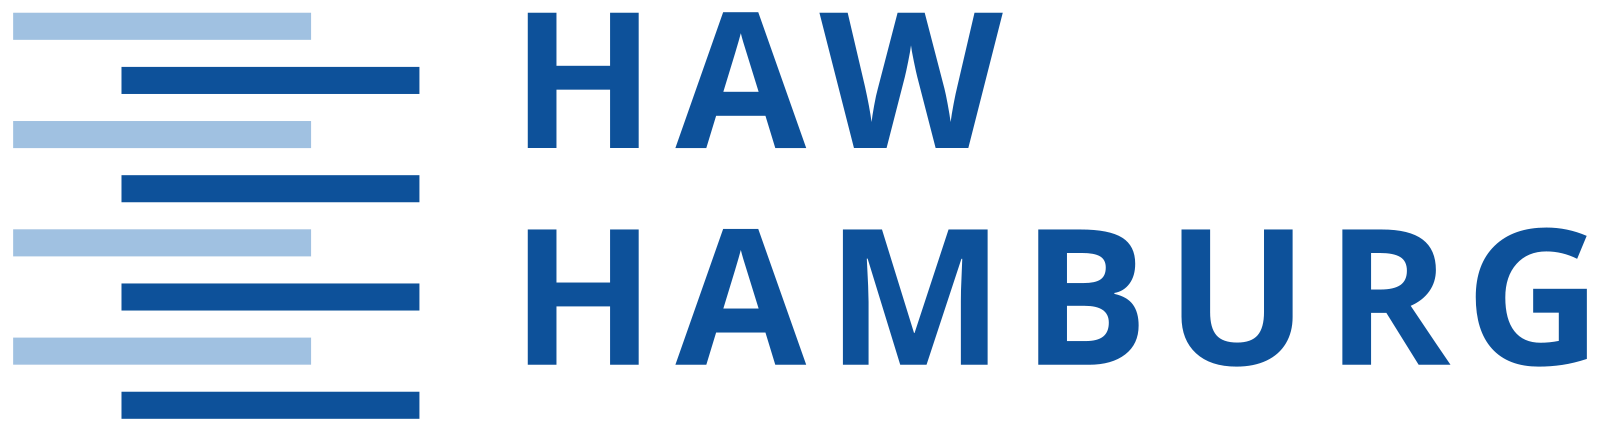
\includegraphics[height=24pt]{HAWLogo}}    % HAW Logo in Kopfzeile einfügen
\lhead{Bussysteme und Sensorik}  % Beschreibung in Kopfzeile

\renewcommand{\footrulewidth}{0.4pt}    % Linie in Fußzeile einfügen
\rfoot{\thepage}    % Seitenzahlen einfügen
\lfoot{Department Informations- und Elektrotechnik}   % Fusszeile linksbündig

\begin{document}
%Titelseite
\begin{titlepage}

  \begin{figure}
    \centering
    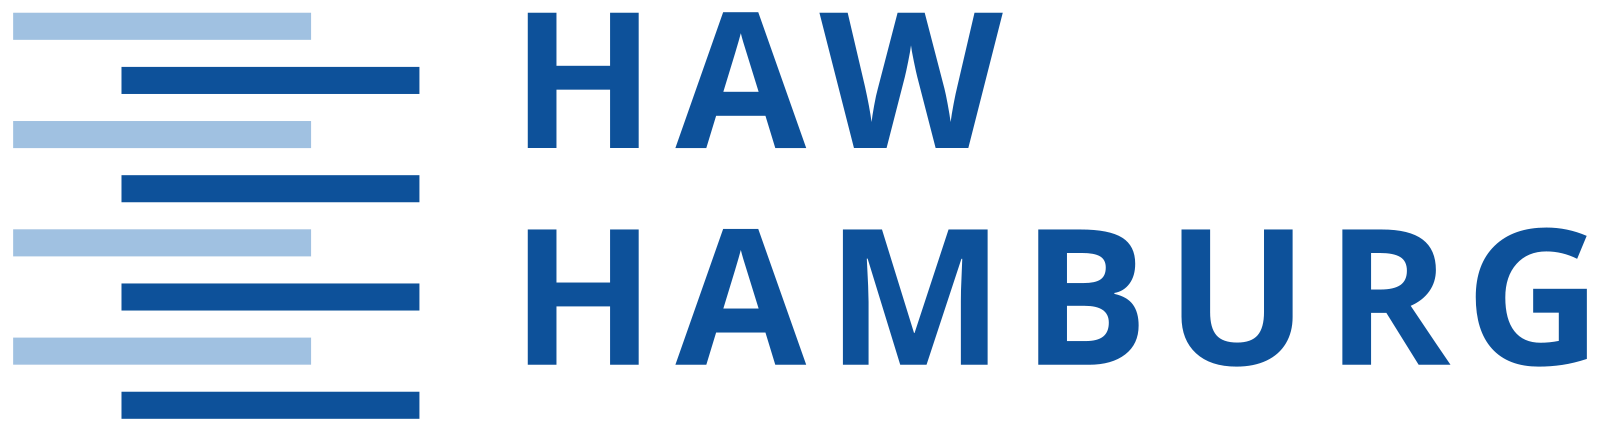
\includegraphics[height=2.5cm]{HAWLogo}
  \end{figure}

  \vspace*{2cm}
  \centering
  {\scshape\Large Bussysteme und Sensorik \par}
  \vspace{1cm}
  {\scshape\LARGE Entwicklung eines Hubs zur Erfassung und graphischen Darstellung von Sensordaten \par}
  \vspace{0.5cm}
  {\scshape\large Wintersemester 2023/2024 \par}
  \vspace{5cm}

  \raggedright
  Ausarbeitung von:

  \vspace{0.5cm}
  Lasse Kelling \\
  123456 % matnr

  \vspace{0.2cm}
  Fabian Schmalenbach \\
  2514071

  \vspace{0.5cm}
  Abgabedatum: 24.01.2024

  \vspace{0.5cm}
  Prüfer: Prof. Dr. R. Fitz



\end{titlepage}

\newpage
\addtocontents{toc}{\protect\thispagestyle{empty}}
\tableofcontents
\thispagestyle{empty}
\newpage

\setcounter{page}{1}    % Seitenzähler sicherheitshalber zurücksetzen

\section{Projektbeschreibung}
\label{sub:projektbeschreibung}

Ziel des Projekts ist die Entwicklung eines Sensorhubs, der Sensordaten erfasst und auf einem Display darstellt.
Bei den Sensoren handelt es sich in erster Linie um Umweltdaten, die aktuelle Parameter der Umgebung erfassen.
Das Projekt kann daher grob mit einer Wetterstation verglichen werden.

\subsection{Anforderungen}
\label{subsub:anforderungen}

Es wurden keine verpflichtenden Anforderungen gestellt, das Projekt soll thematisch aber zum Modul
"Bussysteme und Sensorik" passen. Daraus lassen sich für das spezifische Projekt Anforderungen stellen bzw. ableiten:

\begin{itemize}
  \item Verwendung eines oder mehrerer Bussysteme zur Kommunikation zwischen Mikrocontrollern
  \item Nutzung diverser Sensoren mit unterschiedlichen Anbindungen für Vielfältigkeit
  \item Analog zu herkömmlichen Wetterstationen, soll diese ebenfalls über einen Außensensor verfügen
  \item Die Wetterstation soll über eine Wettervorhersage verfügen
  \item Der Sensorhub soll skalier- und erweiterbar sein
\end{itemize}

\noindent
Aus diesen Anforderungen lassen sich direkt Vorgaben für das Projekt ableiten:
\begin{itemize}
  \item Nutzung mehrerer Mikrocontroller, die miteinander über ein Bussystem kommunizieren
  \item Verwendung digitaler Sensoren, die Standardprotokolle wie I2C, SPI oder UART unterstützen
  \item Entwicklung eines Außensensors, der drahtlos mit dem Sensorhub kommunizieren kann
  \item Anbindung des Sensorhubs ans Internet oder Empfang von Wettervorhersagen via Funk (DCF77)
  \item Nutzung ausreichend leistungsstarker Mikrocontroller, die genügend Leistungs- und Peripheriereserven haben, um weitere Geräte anzubinden
\end{itemize}

\section{Systembeschreibung}
\label{sub:systembeschreibung}

\subsection{Systemaufbau}
\label{subsub:systemaufbau}

\begin{figure}[H]
  \centering
  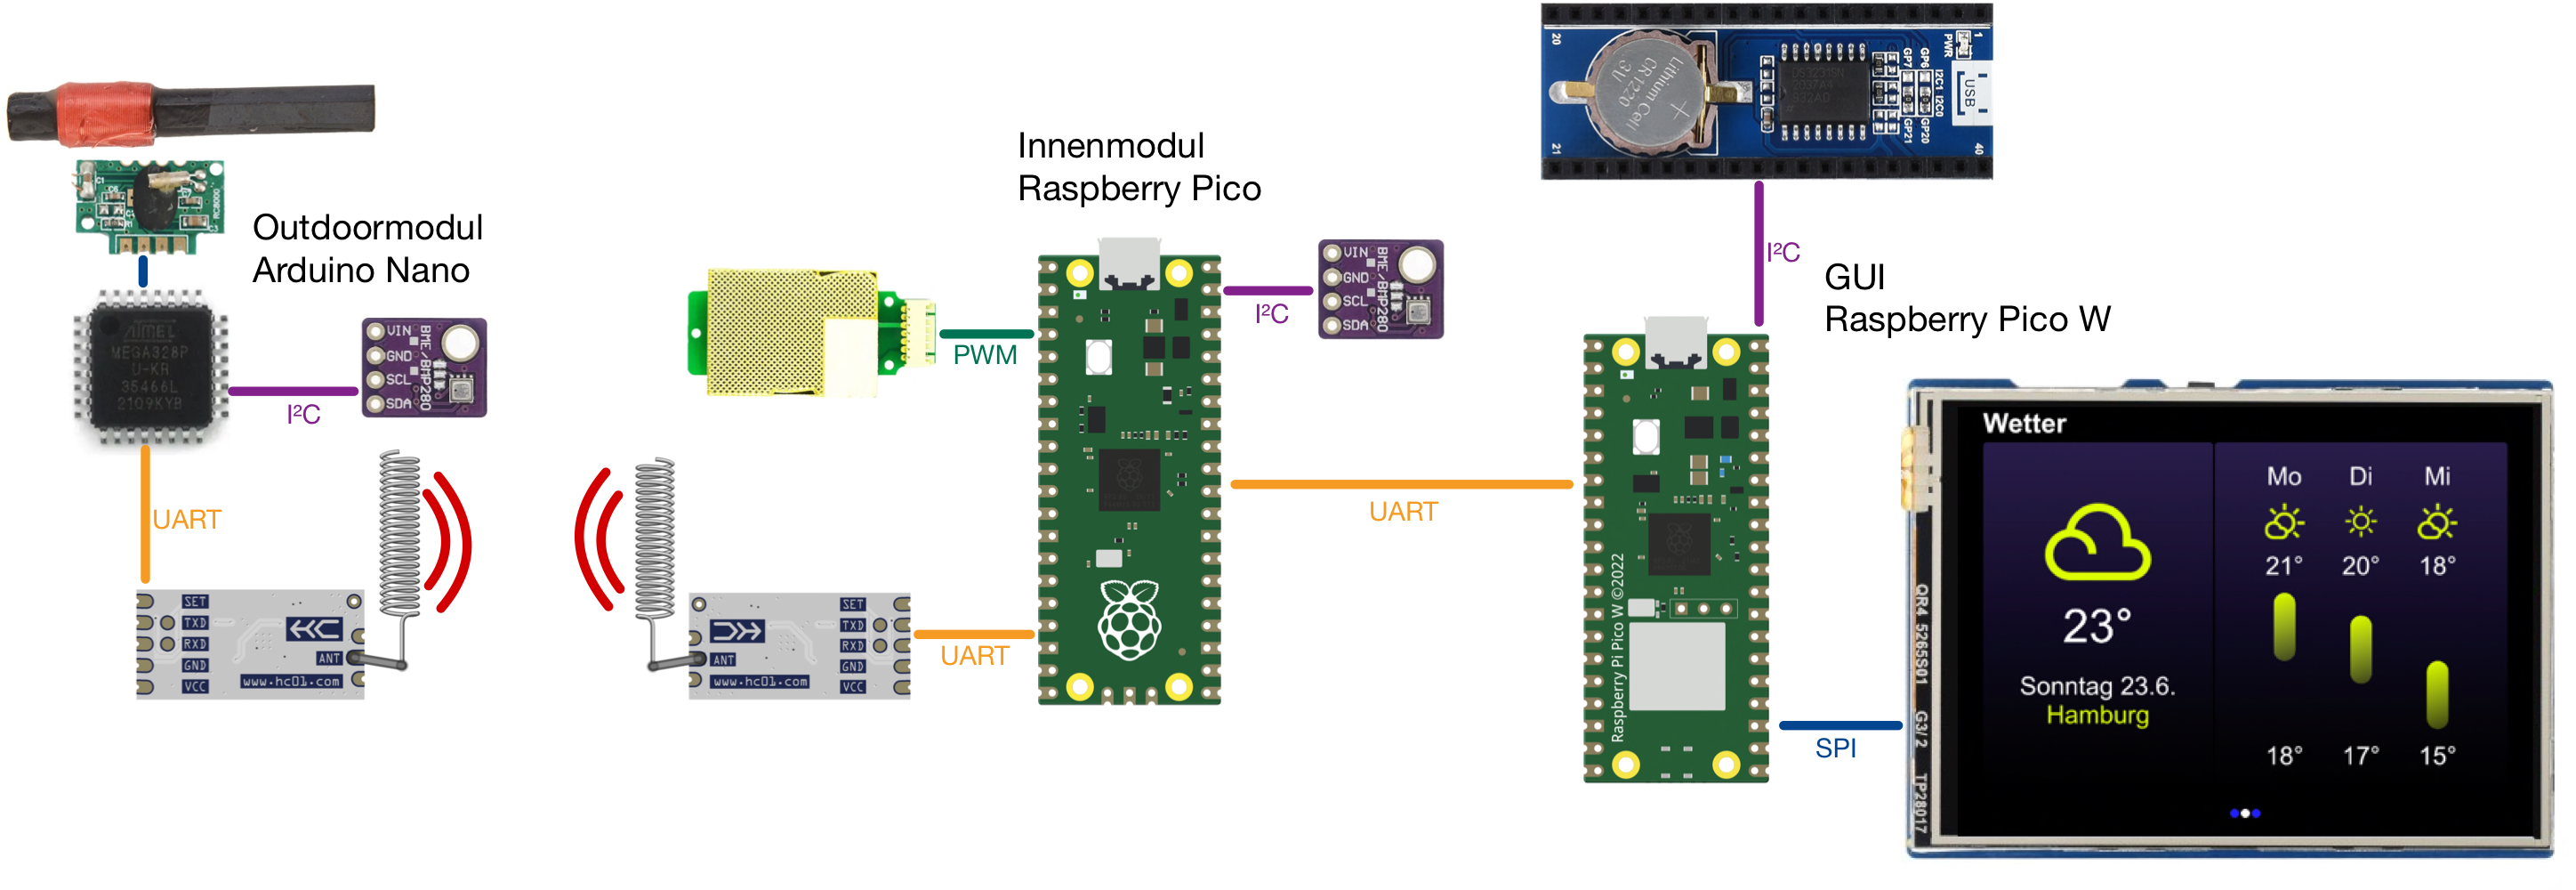
\includegraphics[width = 0.8\textwidth]{Systemuebersicht}
  \caption{Übersicht der Systemkomponenten}
  \label{fig:systemuebersicht}
\end{figure}

Die obige Abbildung \ref{fig:systemuebersicht} zeigt abstrakt alle Komponenten des Systems. Die jeweiligen Komponenten über dem Mikrocontroller Symbol
zeigen jeweils die angeschlossenen Sensoren bzw. Bildschirme. Ebenfalls ist grob die Kommunikation zwischen den Mikrocontrollern erkennbar. 

\vspace{0.2cm}
\noindent
Ganz links ist der Außensensor dargestellt, an den ein Sensor zur Messung von Temperatur, Luftfeuchtigkeit und Luftdruck angeschlossen ist. 
Außerdem verfügt dieser über eine Antenne, um das DCF77-Signal zu empfangen, welches die aktuelle Zeit und eine Wettervorhersage beinhaltet (siehe Abschnitt \ref{subsubsub:dcf77}).
Der Sensor sendet die empfangenen Daten zyklisch per 433 MHz Sender an den Sensorhub. 

\vspace{0.2cm}
\noindent
Der Sensorhub besteht aus zwei Mikrocontrollern, die über eine serielle Schnittstelle (UART) miteinander kommunizieren. Der in Abbildung \ref{fig:systemuebersicht} mittlere Mikrocontroller
empfängt die Daten des Außensensors und leitet diese weiter an den verbundenen Mikrocontroller. Da die Daten zur Wettervorhersage verschlüsselt sind und der Außensensor möglichst
wenig Energie verbrauchen soll, müssen die Daten vom Mikrocontroller entschlüsselt werden. Dazu werden die entsprechenden Datenpakete abgefangen, entschlüsselt und anschließend weitergesendet. 
Der Mikrocontroller verfügt außerdem wie der Außensensor über einen Sensor zur Messung von Temperatur, Luftfeuchtigkeit und Luftdruck (wobei der Luftdruck im Innenraum nicht gemessen wird). 
Zusätzlich ist ein CO2 Sensor verbaut, der die Konzentration im Raum misst. 

\vspace{0.2cm}
\noindent
In der Übersicht ganz rechts ist der Mikrocontroller, der alle Daten empfängt und auf einem Touchdisplay darstellt. Da der Sensor über ein WLAN-Modul verfügt, wäre theoretisch
zusätzlich die Übertragung der Daten per WLAN an einen Server o.ä. möglich, der alle Daten speichert und diese anderen Geräten zur Verfügung stellt. 

\subsection{Sensorik}
\label{subsub:sensorik}

Zur Erfassung der Umweltparameter werden aktuell zwei verschiedene Sensoren eingesetzt. Der BME280 erfasst Lufttemperatur, Luftfeuchtigkeit und Luftdruck. 
Der MHZ19C wird zur Erfassung der CO2 Konzentration im Raum eingesetzt. In den folgenden beiden Abschnitten werden die Sensoren beschrieben. 

\vspace{0.2cm}
\noindent
Das Außenmodul verfügt außerdem über eine 77,5 kHz Empfangsantenne, um das Zeitzeichensignal DCF77 zu empfangen. Daraus lässt sich die aktuelle Zeit ablesen,
außerdem wird eine Wettervorhersage mit übertragen, die ausgewertet wird. 

\subsubsection{BME280}
\label{subsubsub:bme280}

Beim BME280 handelt es sich um einen effizienten Sensor von Bosch, der zur Erfassung von Temperatur, Luftfeuchtigkeit und Luftdruck eingesetzt wird. 
Der Sensor verfügt über ein I2C und SPI Interface.
Beim zyklischen Auslesen aller Sensordaten mit 1 Hz liegt die Stromaufnahme laut Datenblatt bei 3,6 $\mu$A, weshalb sich der Sensor ideal für die Anwendung in Sensormodulen mit Batteriebetrieb eignet. 

Der Sensor verfügt über die folgenden Messbereiche:
\begin{itemize}
  \item Temperatur: -40°C - +85°C ($\pm$ 0,5°C)
  \item Luftfeuchtigkeit: 0 - 100\% rel. Feuchtigkeit ($\pm$ 3\%)
  \item Druck: 250 - 1250 hPa ($\pm$ 1 hPa)
\end{itemize}

\noindent
Mit diesen Spezifikationen eigent sich der Sensor für die Anwendung im Innen- und Außenbereich. 

\noindent
Für das Projekt wird ein Sensorshield verwendet, welches nur den I2C Bus herausführt. Die Ansteuerung des Sensors erfolgt daher über I2C. 

\subsubsection{MHZ19C}
\label{subsubsub:mhz19c}

Der MHZ-19C ist ein Infrarot CO2-Sensor, der die CO2 Konzentration mittels nicht-dispersiver Infrarot-Spektroskopie misst. Dabei wird zyklisch mit einer Infrarotlampe
und einem Photosensor die CO2-Konzentration anhand der Reflexion des Lichts durch CO2 Partikel gemessen. 
Der Sensor verfügt über einen Messbereich von 400-5000 ppm, wobei die Genauigkeit $\pm$ 40ppm + 5\% des Messwerts beträgt. 
Da NDIR Sensoren zum Messwertdrift neigen, verfügt der Sensor über eine automatische Kalibrierung, die alle 24 Stunden erfolgt. Der Sensor ist daher für den Dauerbetrieb ausgelegt
und sollte dauerhaft aktiv sein. 
Die Aufheizzeit des Sensors beträgt eine Minute. 

\noindent
Der Sensor ist über eine UART-Schnittstelle konfigurier- und auslesbar, außerdem verfügt er über einen PWM Ausgang. 

\subsubsection{DCF77}
\label{subsubsub:dcf77}

Bei DCF77 handelt es sich um einen Zeitzeichensender in der Nähe von Frankfurt am Main, welcher mit einer Trägerfrequenz von 77,5 kHz ein Zeitsignal überträgt. 
Das Signal ist europaweit empfangbar und wird von den meisten Funkuhren als Referenzsignal verwendet.  

\noindent
Die Datenübertragung erfolgt durch einfache Amplitudenmodulation, indem die Amplitude für eine Dauer von 100 ms (Bit 0) oder 200 ms (Bit 1) auf 25\% der Ausgangsamplitude abgesenkt wird. 
Damit wird eine Bitrate von 1 Bit pro Sekunde erreicht. 

\begin{figure}[H]
  \centering
  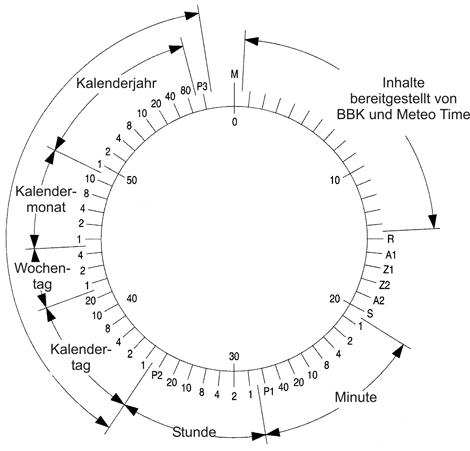
\includegraphics[width=0.7\textwidth]{dcf77Code}
  \caption{Kodierungsschema der DCF77 Zeitinformationen \\
           \url{https://www.ptb.de/cms/ptb/fachabteilungen/abt4/fb-44/ag-442/verbreitung-der-gesetzlichen-zeit/dcf77/zeitcode.html}}
  \label{fig:dcf77Schema}
\end{figure}

\noindent
Abbildung \ref{fig:dcf77Schema} zeigt die Kodierung aller Datenbits innerhalb einer Minute. Daraus ist erkennbar, dass ein Datenpaket 59 Bits lang ist und
die Übertragung eine Minute dauert. Ein Paket beginnt zu jeder neuen Minute. In der letzten Sekunde einer Minute erfolgt keine Absenkung des Trägers, sodass anhanddessen
das Ende eines Pakets abgeleitet werden kann. 

\vspace{0.2cm}
\noindent
Die neue Minute beginnt mit dem nullten Bit, das immer den Wert null hat. Darauf folgen 14 Bits mit verschlüsselten Wetterinformationen der Firma MeteoTime.
Diese werden im nächsten Abschnitt weiter beschrieben. \\
Bit 15 (R) ist ein Rufbit, dass zur Alarmierung der PTB Mitarbeiter dient, wenn Unregelmäßigkeiten vorliegen. \\
Bit 16 (A1) zeigt an, dass am Ende der Stunde ein Wechsel von Sommer- zu Winterzeit stattfindet. \\
Bit 17 (Z1) ist eine Flag für die Sommerzeit. \\
Bit 18 (Z2) ist eine Flag für die Winterzeit. \\
Bit 19 (A2) zeigt an, dass am Ende der Stunde eine Schaltsekunde eingefügt wird. \\
Bit 20 (S) markiert den Beginn der Zeitinformationen und hat den Wert eins. 

\vspace{0.2cm}
\noindent
Wie schon aus der Abbildung hervorgeht, werden in den restlichen Sekunden Informationen zu Zeit und Datum übertragen, Minute, Stunde und Datum haben jeweils ein
Paritätsbit eingefügt, um Fehler erkennen zu können. Eine Fehlerkorrektur ist damit allerdings nicht möglich. 

\subsubsubsection{MeteoTime}
\label{subsubsubsub:meteotime}

MeteoTime versendet versendet pro Minute 14 Bits mit Wetterinformationen, die von lizensierten Geräten entschlüsselt- und verwendet werden können. 
Ein Informationspaket besteht aus 42 Bits und benötigt für die Übertragung somit drei Minuten. Ein Tag ist in fünf Abschnitte unterteilt, in denen
unterschiedliche Informationen übertragen werden. Da die Wettervorhersage 90 Regionen abdeckt, wird jede Vorhersage nur täglich einmal übertragen. \\
Es gilt folgende Aufteilung: \\
22:00 Uhr - 03:59 Uhr: Aktueller Tag \\
04:00 Uhr - 09:59 Uhr: Folgender Tag \\
10:00 Uhr - 15:59 Uhr: Darauffolgender Tag \\
16:00 Uhr - 18:59 Uhr: Darauffolgender Tag \\
19:00 Uhr - 21:59 Uhr: Zusatzregionen mit 2-Tages Prognose. 

\vspace{0.2cm}
\noindent
Von den 90 Regionen erhalten 60 die viertägige Vorhersage, die restlichen 30 Regionen erhalten nur eine 2-Tages Vorhersage. \\
Innerhalb eines sechsstündigen Übertragungszeitraums werden für jede Region nacheinander die Höchst- und Tiefstwerde übertragen.

\noindent
Die Wettervorhersagen decken große Regionen ab, weshalb diese etwas ungenau sind. \\
Für Hamburg ist beispielsweise die Region Bremerhaven zugeteilt, der Bereich deckt alles vom westlichen Schleswig-Holstein bis zum Nordwesten der Niederlande ab. \\
Um im Fall eines Lesefehlers beim Empfang der Daten trotzdem eine Vorhersage ableiten zu können, sollten Ausweichregionen definiert werden, die im Fehlerfall stattdessen angezeigt werden. \\
Für Hamburg sind das die Regionen Rostock und Hannover. 

\vspace{0.3cm}
\noindent
Für die Entschlüsselung der Wetterinformationen ist ein Dekodier-IC notwendig, welches vermutlich aus rückgekoppelten Schieberegistern besteht, um die Daten zu Dekodieren. \\
Beim IC handelt es sich um das Modell HKW581 der Firma HKW, die auch Betreiber des MeteoTime Dienstes ist. 

\begin{figure}[H]
  \centering
  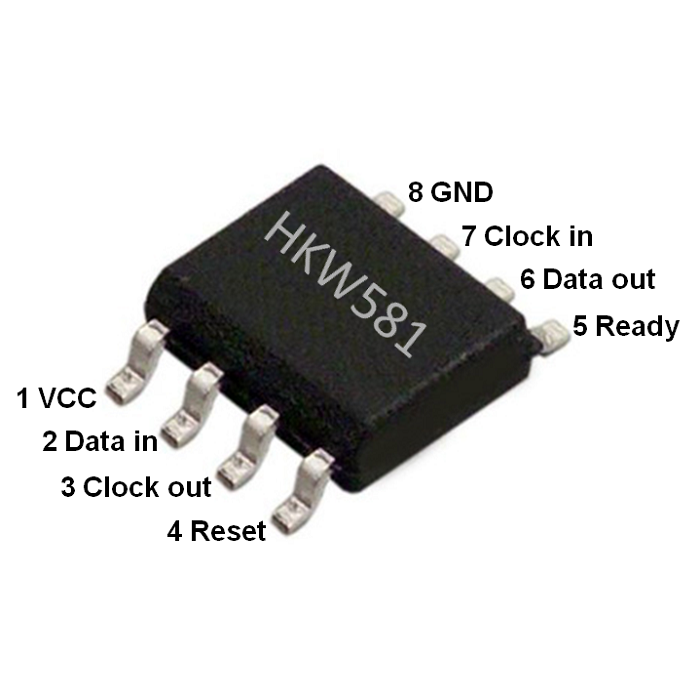
\includegraphics[width = 0.2\textwidth]{HKW5811}
  \caption{Dekodier-IC zum Entschlüsseln der Wettervorhersagen}
  \label{fig:hkw581}
\end{figure}

\noindent
Der IC verfügt über acht Pins, davon sind neben den Pins zur Spannungsversorgung und Daten Ein- und Ausgabe auch ein Clock IN und Clock OUT Pin vorhanden, damit die Bits
taktsynchron ein- bzw. ausgelesen werden. Der Clock OUT Pin folgt dem Clock IN Pin und wird zur Indikation genutzt, ob am Datenausgang ein valider Bitwert anliegt. 
Neben einem Resetpin gibt es außerdem einen Ready Pin, der anzeigt, dass der IC betriebsbereit ist. Anscheinend braucht der IC eine Aufwärmphase. 

\vspace{0.2cm}
\noindent
Als Eingabedaten benötigt der IC einen 82 Bit langen Datenstream, der sich wie folgt zusammensetzt:
\begin{itemize}
  \item Meteopaket 1 (14 Bit)
  \item Meteopaket 2 (14 Bit)
  \item Meteopaket 3 (14 Bit)
  \item Minute des ersten Pakets (aufgefüllt von 7 auf 8 Bit)
  \item Stunde des ersten Pakets (aufgefüllt von 6 auf 8 Bit)
  \item Kalendertag (aufgefüllt von 6 auf 8 Bit)
  \item Monat (5 Bit)
  \item Wochentag (3 Bit)
  \item Jahr (8 Bit)
\end{itemize}

\noindent
Als Ausgabe erhält man einen 22 Bit langen Datenstream mit den Wetterinformationen. Je nachdem, ob gerade ein Paket mit Höchst- oder Tiefstwerten gesendet wurde, 
ergeben sich unterschiedliche Informationen:

\vspace{0.2cm}
\noindent
Höchstwerte:
\begin{itemize}
  \item Wetter Tag (4 Bit)
  \item Wetter Nacht (4 Bit)
  \item Schweres Wetter (4 Bit)
  \item Niederschlagswahrscheinlichkeit(3 Bit)
  \item Wetteranomalie Tag (1 Bit)
  \item Temperatur Tag (6 Bit)
\end{itemize}

\vspace{0.2cm}
\noindent
Tiefstwerte:
\begin{itemize}
  \item Wetter Tag (4 Bit)
  \item Wetter Nacht (4 Bit)
  \item Windrichtung (4 Bit)
  \item Windstärke (3 Bit)
  \item Wetteranomalie Nacht (1 Bit)
  \item Temperatur Nacht (6 Bit)
\end{itemize}

\noindent
Die ausgegebenen Zahlenwerte sind wiederum einer Bezeichnung zugeordnet (z.B. Wetter Tag = 3 entspricht vorwiegend bewölkt).

\subsection{Kommunikation}
\label{subsub:kommunikation}

Die Kommunikation zwischen den Mikrocontrollern erfolgt sowohl kabelgebunden, als auch drahtlos. Für die kabelgebundene Kommunikation wird UART mit einer Baudrate
von 115200 bd genutzt. Die Drahtloskommunikation erfolt über einen 433 MHz Transmitter und Receiver, die jeweils über UART beschrieben und gelesen werden können. 

\subsubsection{Funkstrecke}
\label{subsubsub:funkstrecke}

Bei den Funkmodulen handelt es sich um "HC-12 Wireless RF communicatio module V2.4" Module. Diese versprechen eine Übertragungsdistanz von bis zu 1800 m
und eine einfache Ansteuerung über UART. \\
Die Module haben eine Sendeleistung von bis zu 100 mW und können auf 100 verschiedenen, einstellbaren Kanälen funken (433,4 MHz bis 473 MHz). Die Baudrate ist einstellbar
zwischen 1200 bps und 115200 bd. 

\vspace{0.5cm}
\noindent
Aufgrund der geltenden Bestimmungen in Deutschland darf nur mit maximal 10 mW gesendet werden, auch ist der wählbare Frequenzbereich teilweise nicht legal.
Es können nur die Kanäle 1 bis 4 genutzt werden. 

\subsubsection{Datenpakete}
\label{subsubsub:datenpakete}

Je nach übertragener Information werden unterschiedliche Datenpakete verwendet, die zur Identifikation jeweils mit einem 4-Byte langen Identifier ausgestattet sind. \\
Aktuell gibt es fünf verschiedene Identifier:
\begin{itemize}
  \item "IBME" Internal BME
  \item "EBME" External BME
  \item "CO2." Co2 Konzentration
  \item "TIME" Aktuelle Zeit
  \item "MTEO" Wettervorhersage
\end{itemize}

Die Datenpakete haben unterschiedliche Längen und sind in Form von Structs in C definiert. Zum Senden der Date werden diese dann in char arrays umgewandelt. 

\section{Modulbeschreibung}
\label{sub:modulbeschreibung}

\subsection{Sensormodul extern}
\label{subsub:sensorModul_ext}

\subsection{Sensormodul intern}
\label{subsub:sensorModul_int}

\subsection{Grafikmodul}
\label{subsub:grafikmodul}

\section{Aktueller Projektstand}

\end{document}
